\chapter{Methoden}\label{ch:methods}

Zur Pose Estimation werden zwei separate Funktionen benötigt: Object Detection der Hand und anschließend die Lokalisierung der Keypoints.
Für die erste Aufgabe wird ein YOLOv5 Modell \cite{yolov5} und ein FasterRCNN Modell \cite{fasterrcnn} verglichen, welche potenziell Austauschbar sind.
Die Lokalisierung der Keypoints übernehmen dabei selbst kreierte Modelle, die für die spezifischen Handtypen ausgelegt sind.
Abbildung \ref{fig:arch} zeigt eine Übersicht der beschriebenen Architektur. \\
\begin{figure}[!htb]
    \centering
    \fbox{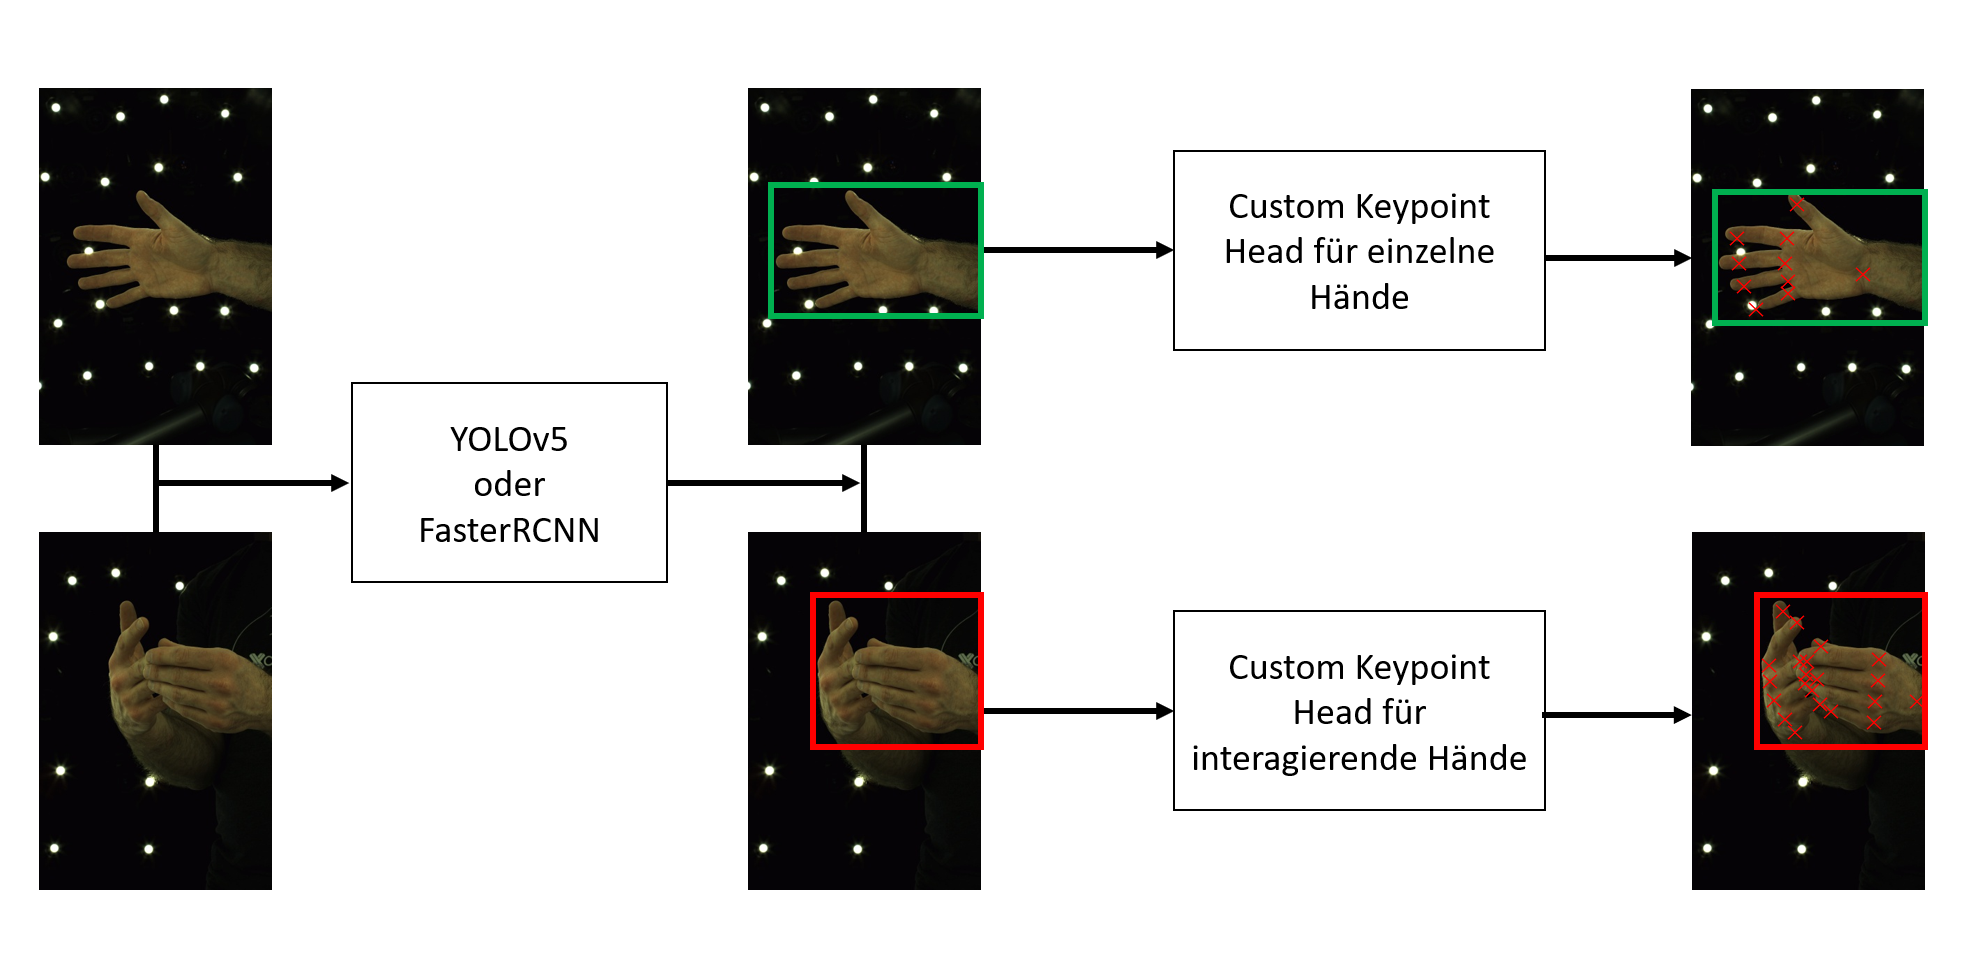
\includegraphics[width=15.5cm]{abbildungen/arch.PNG}}
    \caption{Übersicht Architektur}
    \label{fig:arch}
\end{figure} 

Als Alternative zu dieser Architektur, wird noch ein KeypointRCNN \cite{keypointrcnn} trainiert.
Dabei handelt es sich um Abwandlung von MaskRCNN, eine Weiterentwicklung der FasterRCNN Architektur, welche ursprünglich für Image Segmentation entwickelt wurde.
Diese Architektur wird detailliert in Kapitel \ref{ch:keypointrcnn} beschrieben.

\section{Dataset}\label{ch:dataset}
Die Bilder des InterHand2.6M Datensatz können über ein Python Skript, zu finden unter scripts/download\_data.py, heruntergeladen werden. 
Die Annotation müssen jedoch separat über die InterHand2.6M Website \cite{interhand_website} heruntergeladen werden. \\

Die Daten können als ein PyTorch Dataset geladen werden.
Dabei werden alle Annotationen geladen und vorverarbeitet. 
Während der Laufzeit werden die Bilder erst aus dem Filesystem geladen, was Ressourcen wie den Arbeitsspeicher schont. \\
\begin{lstlisting}[language=Python,caption={Dataset},label={lst:dataset},captionpos=b,showstringspaces=false, basicstyle=\small]
from dataset import dataset
data = dataset.Dataset(mode='train',
                    transform = None,
                    only_keypoints = False,
                    limit_handedness = 'all')
\end{lstlisting}
Die Keypoints der jeweiligen 2D Bilder sind nicht direkt in den Annotationen gespeichert.
Stattdessen sind Informationen über die Kameraposition (Kameramatrix) und die globalen 3D Koordinaten enthalten.
Mithilfe dieser, können die Keypoints auf das 2D Bild projiziert werden.\\
Über den Parameter 'mode' kann gesteuert werden, welcher der Datensätze (Train, Test oder Val) geladen werden soll.
Zusätzlich kann 'limit\_handedness' dazu genutzt werden, um nur Hände eines bestimmten Typs (interagierend, einzeln, links oder rechts) in dem Datensatz zu berücksichtigen.
Als Standard 'transform' wird eine Konvertierung zu einem PyTorch Tensor genutzt, jedoch kann bei Bedarf auch bspw. ein Resize übergeben werden.\\
Je nach Modell muss der Parameter 'only\_keypoints' gesetzt werden.
Ist dieser nicht gesetzt, so wird neben dem Bild als Input, ein Dict als Target übergeben.
Dieses ist im COCO Format \cite{coco} und enthält unter anderem Felder über die Bounding-Box der Hände, das Label der Hände und die Keypoints der Hände.\\
Ist der Parameter auf True gesetzt, so wird das Bild um die Bounding-Box herum ausgeschnitten.
Somit fällt der Großteil des Hintergrunds weg.
Zusätzlich werden die Keypoints der Hände normalisiert, d.h. diese haben einen Wert zwischen 0 und 1, je nachdem wie weit diese von den Rändern entfernt sind.
Ist das ausgeschnittene Bild zum Beispiel 500x500 Pixel groß und ein Keypoint befindet sich an Pixel [100 , 200] in diesem Ausschnitt, so wird dieser als [0.2 , 0.4] kodiert.\\

Das YOLOv5 Modell benötigt nicht als PyTorch Dataset, sondern in einer einzigen Ordnerstruktur.
Über das Skript scripts/create\_yolo\_annotations.py kann diese Ordnerstruktur erzeugt werden.
Jedoch benötigt dieser Vorgang ziemlich viel Zeit, da das Filesystem (Windows) nicht mit so viele Daten in einem einzigen Order zurechtkommt.
Die Erstellung des Val-Datensatzes mit ca. 380k Bildern benötigte nur eine halbe Stunde, wohingegen der Train-Datensatz knapp 45 Stunden brauchte, 90 mal solange trotz des eigentlich nur 3 mal so großen Datenmenge.

\section{YOLOv5}
YOLO steht für You Only Look Once, was auch direkt eine Besonderheit dieses Object Detection Networks ausmacht: Es reicht ein einziger Durchlauf des Bildes durch das Modell \cite{yolo1}.
In diesem Durchlauf, wird das Bild in ein Grid der Größe \textit{S x S} eingeteilt. 
Ist der Mittelpunkt einer Label-Bounding-Box in dieser Zelle, so ist diese Verantwortlich das Objekt zu erkennen.
Dabei werden \textit{B} Bounding Boxen in verschiedenen Größen und Längen-Breiten-Verhältnissen gebildet. 
Diese enthalten neben der Mittelpunkt, sowie Höhe und Breite der Box, noch den Confidence Score für entsprechendes Objekt.
Abbildung \ref{fig:yolo1_bbox} zeigt, wie diese Bounding Boxen auf einem Beispielbild aussehen.\\
\begin{figure}[!htb]
    \centering
    \fbox{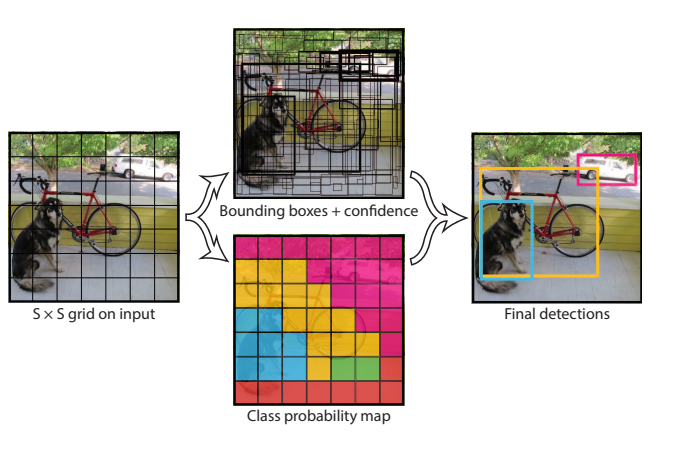
\includegraphics[width=10cm]{abbildungen/yolo1_bbox.PNG}}
    \caption{Bounding Box Erkennung YOLO \cite{yolo1} }
    \label{fig:yolo1_bbox} 
\end{figure} 

YOLO sagt dies Koordinaten dieser Bounding Boxen direkt im Forward-Pass des Modells vorher, was in der Architektur in Abbildung \ref{fig:yolo1_arch} ersichtlich ist.
Als Feature Network werden einige Convolution Layers genutzt, die anschließend als Input für Fully Connected Layers dienen. 
Diese FC Layers predicted dabei die Koordinaten der Bounding Boxes.\\
\begin{figure}[!htb]
    \centering
    \fbox{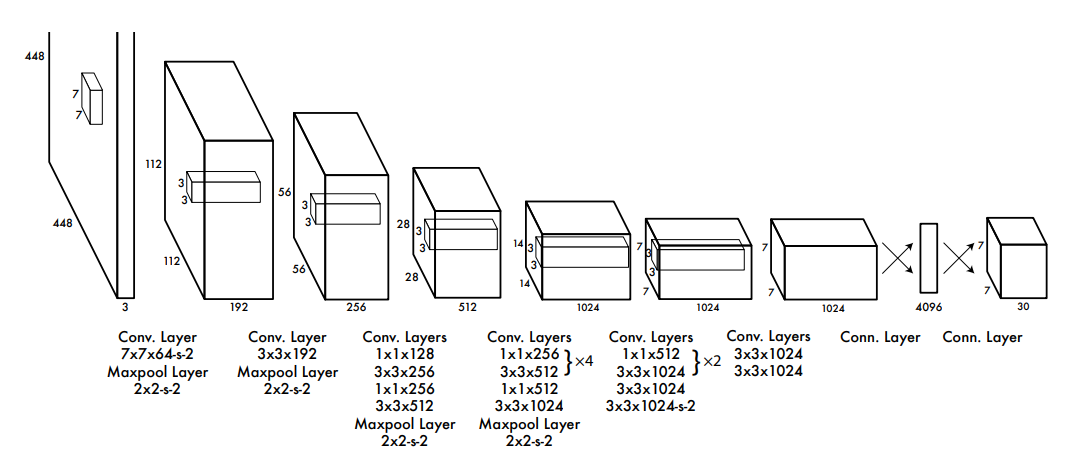
\includegraphics[width=15.5cm]{abbildungen/yolo1_arch.PNG}}
    \caption{Architektur YOLO \cite{yolo1} }
    \label{fig:yolo1_arch}
\end{figure} 

YOLOv5 ist eine Weiterentwicklung des ursprünglichen YOLO Modells.
Diese enthält diversen Verbesserungen, die teils auch über die vorherigen YOLO Varianten hinzugefügt wurden
So werden bspw. seit YOLO9000 (YOLO2) eine Optimierung der Bounding Box Vorschläge, sogenannte Anchor Boxen, genutzt \cite{yolo2}.
Die wichtige Neuerung von YOLO in Version Nummer 5 ist die Verwendung eines CSP Backbone.
Dabei handelt es sich um Convolutional Layers, bei denen einzelne Layers mehrfach verwendet werden.
Ziel dabei ist es, das Netzwerk dazu zu bringen Features wiederzuverwenden, sowie Probleme wie das Vanishing Gradient Problem zu verringern.\\

Um YOLOv5 zu trainieren, muss zuerst der Preprocessing Step aus Kapitel \ref{ch:dataset} ausgeführt werden.
Anschließend muss eine Konfiguration als .yaml Datei erzeugt werden, welche sich bereits unter yolo\_data/yolo\_dataset.yaml befindet.
Diese enthält neben den Pfad zu den Datensätzen auch die Labels der Klassen.
Nach dem Klonen des git-Repos, kann das Training über die Konsole gestartet werden.
Alternativ kann das Training auch über das Notebook Training.ipynb ausgeführt werden (dieses führt bei Bedarf auch nur den Konsolenbefehl aus).

\begin{lstlisting}[language=bash,caption={YOLO Training},label={lst:yolo_train},captionpos=b,showstringspaces=false, basicstyle=\small]
python .\yolov5\train.py --batch 2 --epochs 2 \\
    --data yolo_data/yolo_dataset.yaml \\
    --weights yolov5s.pt --freeze 8
\end{lstlisting}

\section{FasterRCNN}
Eine Alternative zu YOLO bietet die Klasse der RCNN Modelle.
FasterRCNN ist dabei der Nachfolger von FastRCNN und dieses wiederum von RCNN \cite{fasterrcnn}.
Im Gegensatz zu YOLO reicht es jedoch nicht, dass das Bild ein einziges Modell einmal durchläuft.
Stattdessen besteht FasterRCNN aus 3 Teilen: Feature Network, Region Proposal Network und einem Region of Interest Pooling. 
Abbildung \ref{fig:fasterrcnn} zeigt das Zusammenspiel dieser Komponenten. \\
\begin{figure}[!htb]
    \centering
    \fbox{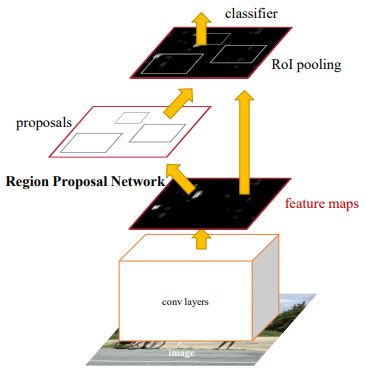
\includegraphics[width=10cm]{abbildungen/fasterrcnn_arch.PNG}}
    \caption{Architektur FasterRCNN \cite{fasterrcnn} }
    \label{fig:fasterrcnn}
\end{figure} 
Als Feature Network dienen einige Convolutional Layers. 
Hier können bereits vortrainierte Modelle (bzw. Convolution Layer dieser Modelle), bspw. ResNet50 genutzt werden.
Das Region Proposal Network (RPN) lässt sogenannte Anchor Boxen in verschiedenen Größe, Längen-Breiten-Verhältnissen und Ausrichtungen über das Bild laufen (wie ein Sliding Window).
Für jede dieser Anchor Boxen wird dabei predicted, ob ein Objekt darin enthalten ist (Vordergrund) oder nicht (Hintergrund).
Das Region of Interest Pooling (ROI Pooling) ist der letzte Schritt vor der Klassifikation.
Diese Schicht ist dabei ähnlich wie ein einfaches Max-Pooling.
Der Output des ROI Pooling kann nun als Input für einen Klassifikator genutzt werden, der die 'Vordergrund'-Objekte nun den richtigen Klassen zuordnet.\\

PyTorch bietet bereits eine Klasse für FasterRCNN Modelle an, welche auch in diesem Projekt genutzt wird.
Für dieses Modell wird ein Dataset im COCO-Format benötigt, welches bereits in \ref{ch:dataset} beschrieben wurde.
Das Notebook Training.ipynb enthält alle Schritte zur Erstellung, Anpassung und zum Trainieren des FasterRCNN Modells für Hände.

\section{Keypoint Head}

Sowohl YOLOv5 als auch FasterRCNN haben als Output eine Bounding Box um die Hände, sowie ein Label um welche Art von Hand (links, rechts oder interagierend) es sich handelt.
Um nun Keypoints zu bestimmen, wird ein neues Modell benötigt.
Dabei handelt es sich um ein Standard Convolutional Network, welches einige Convolutional Layers gefolgt von einigen Dense Layern beinhaltet.
Die Convolutional Layers werden dabei aber von einem VGG16-Net übernommen.
Die Fully Conected Layers werden von Grund auf an trainiert, wobei die Anzahl der Outputs der doppelten Anzahl der Keypoints entspricht.
Dies liegt daran, dass für jeden Keypoint eine x und eine y-Koordinate bestimmt wird.
Tendenziell wäre es möglich für jeden Hand Typen ein eigenes Modell zu trainieren, jedoch wurden lediglich 2 Modelle genutzt: Eines für interagierende Hände (42 Keypoints) und eines für einzelne Hände, egal ob linke oder rechte Hand (21 Keypoints).
Über entsprechende Parameter des PyTorch Dataset (siehe Kapitel \ref{ch:dataset}), wird das gecroppte Bild sowie die normalisierten Keypoints ausgegeben.
Diese werden bei diesen Modellen zum Training genutzt.
Als Loss Funktion wird hierbei ein simpler MeanSquarredError genutzt, als Optimizer dient Adam.

\begin{figure}[!htb]
    \centering
    \fbox{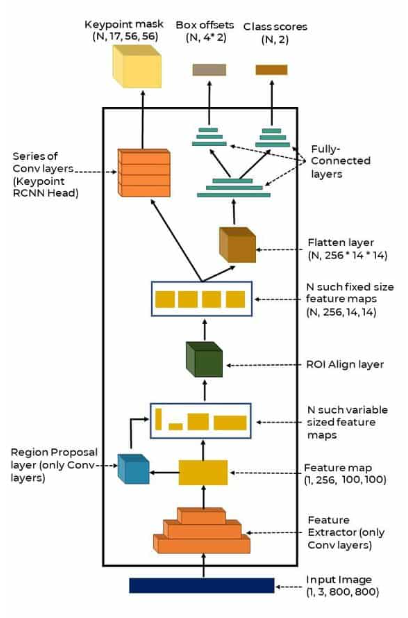
\includegraphics[width=10cm]{abbildungen/keypointrcnn_arch.PNG}}
    \caption{Architektur KeypointRCNN\cite{keypointrcnn_arch} }
    \label{fig:keypointrcnn}
\end{figure} 
\section{KeypointRCNN}\label{ch:keypointrcnn}
Eine Erweiterung der bereits beschriebenen FasterRCNN Architektur ist MaskedRCNN \cite{keypointrcnn}.
Es handelt sich dabei nicht zwingend um eine direkte Weiterentwicklung, da MaskedRCNN nicht für Object Detection sondern für Image Segmentation genutzt wird.
Dabei wird jeder Pixel einer entsprechenden Klasse zugeordnet.
MaskedRCNN baut jedoch auf der FasterRCNN Architektur auf mit einigen Anpassungen.
Anstelle der ROI Pooling Layer besitzt MaskedRCNN eine ROI Align Layer. 
Diese unterscheiden sich durch die Feinheit der weitergegeben Informationen: ROI Pooling nutzt den maximalen Wert, wohingegen ROI Align einen Mittelwert jedes Feldes bildet. 
Dadurch gehen weniger Informationen verloren.
Nach der ROI Align Layer, gibt es noch zusätzlich einen sogenannten MaskedRCNN Head.
Dabei handelt es sich um ein Fully Convolutional Network, bei dem jeder Channel des Outputs einer Klasse entspricht.\\
Eine Variation dieses Netzwerks ist das KeypointRCNN. 
Es besitzt die gleiche Architektur, jedoch ist der Output des MaskedRCNN Heads unterschiedlich.
Anstatt das jeder Channel eine Klasse repräsentiert, kodiert jeder Channel einen Keypoint. 
Abbildung \ref{fig:keypointrcnn} zeigt die Architektur eines KeypointRCNN bei dem 17 Keypoints eines Menschen aus dem COCO Datensatz predicted werden. \\
PyTorch bietet auch hier bereits eine Klasse für KeypointRCNNs an. 
Alle benötigten Schritte zur Modellerstellung und zum Training finden sich ebenfalls in dem Notebook Training.ipynb.


\section{Training}\label{ch:training}
Das Training fand parallel auf 2 Systemen statt: einem privaten Rechner mit einer RTX 2060 Super und einem Hochschulrechner mit einer RTX 2080 Super.
Da der Hochschulrechner eine geteilte Ressource ist, wurde das Training teilweise abgebrochen (z.B. wenn sich ein Student im Rahmen einer Vorlesung angemeldet hatte), wodurch das ganze Training neu gestartet werden musste.
Um solche Dinge zu vermeiden, wurde die Evaluierung mit dem Validation Datensatz bei FasterRCNN und KeypointRCNN weggelassen.
Beide Modelle trainierten für 4 Epochen, was beim FasterRCNN Modell knapp 100 Stunden und beim KeypointRCNN Modell knapp 200 Stunden benötigte. Auch die Custom Keypoint Modelle wurden nur über 5 Epochen trainiert.\\


